\chapter{Patrones GoF}

\section{Introducción}

Estos 23 patrones de diseño son los patrones más conocidos y usados en la actualidad en el campo del Diseño Orientado a Objetos. \newline
En el año 1994, que apareció el libro “Design Patterns: Elements of Reusable Object Oriented Sofware” escrito por los ahora famosos Gang of Four (GoF, que en español es la pandilla de los cuatro) formada por Erich Gamma, Richard Helm, Ralph Johnson y John Vlissides. Los integrantes de la pandilla de los cuatro recopilaron y documentaron 23 patrones de diseño aplicados usualmente por expertos diseñadores de software orientado a objetos. Desde luego que ellos no son los inventores ni los únicos involucrados, pero ese fue luego de la publicación de ese libro que empezó a difundirse con más fuerza la idea de patrones de diseño. \newline
Los patrones de diseño el grupo de GoF clasifican en 3 grandes categorías basadas en su propósito: creacionales, estructurales y de comportamiento. \cite{gof}

“Los patrones de diseño son el esqueleto de las soluciones a problemas comunes en el desarrollo de software.”, es decir,  los patrones de diseño brindan una solución ya probada y documentada a problemas de desarrollo de software que están sujetos a contextos similares. 
Cuando se habla de un patrón de diseño es necesario tener presente los siguientes elementos que lo conforman: 
\begin{itemize}
	\item Nombre
	\item Problema: Define cuando se debe aplicar el patrón.
	\item Solución: Descripción abstracta de la respuesta que soluciona el problema.
	\item Consecuencias: Beneficios y costos de hacer el uso del patrón.
\end{itemize}  


Los patrones se pueden clasificar en tres categorías como se muestra a continuación:

\begin{itemize}
	\item Patrones Creacionales: Instanciación de objetos.
	\item Patrones Estructurales: Separan la interfaz de la implementación.
	\item Patrones de Comportamiento: Caracterizan las formas en  	las que interactúan y reparten responsabilidades las distintas clases u objetos.
\end{itemize}
\newpage




\section{Patrones Creacionales}
\paragraph{Definición}
Los patrones de diseño creacionales proporcionan ayuda a la hora de crear objetos apoyando el proceso de la toma de decisiones, incluso cuando esta toma de decisiones sea de forma dinámica. Además que tratan con las formas de crear instancias de objetos. El objetivo de estos patrones es de abstraer el proceso de instanciación y ocultar los detalles de cómo los objetos son creados o inicializados.
\paragraph{Tipos de Patrones}
Los patrones que se encuentran en la lista de Patrones Creacionales en el enfoque GOF son:
\begin{enumerate}
	\item Abstract Factory (Fábrica Abstracta)
	\item Factory Method (Método Fabrica)
	\item Prototype (Prototipo)
	\item Builder (Constructor)
	\item Singleton (Instancia Única)
\end{enumerate}


\subsection{Fabrica Abstracta}
\subsubsection{Modelo}

El patrón \textbf{Abstract Factory o Fábrica Abstracta} resuleve el problema de crear familias de objetos. Permite trabajar con objetos de diferentes familias de manera que no se mezclen entre sí. El patrón Abstract Factory, por tanto, se recomienda cuando se determina la inclusión de nuevas familias de productos en un futuro, pero resultaría contraproducente si que necesita añadir nuevos productos o modificar los existentes, ya que tendría repercusión en todas las familias creadas.

\begin{figure}[th!]
	\centering
	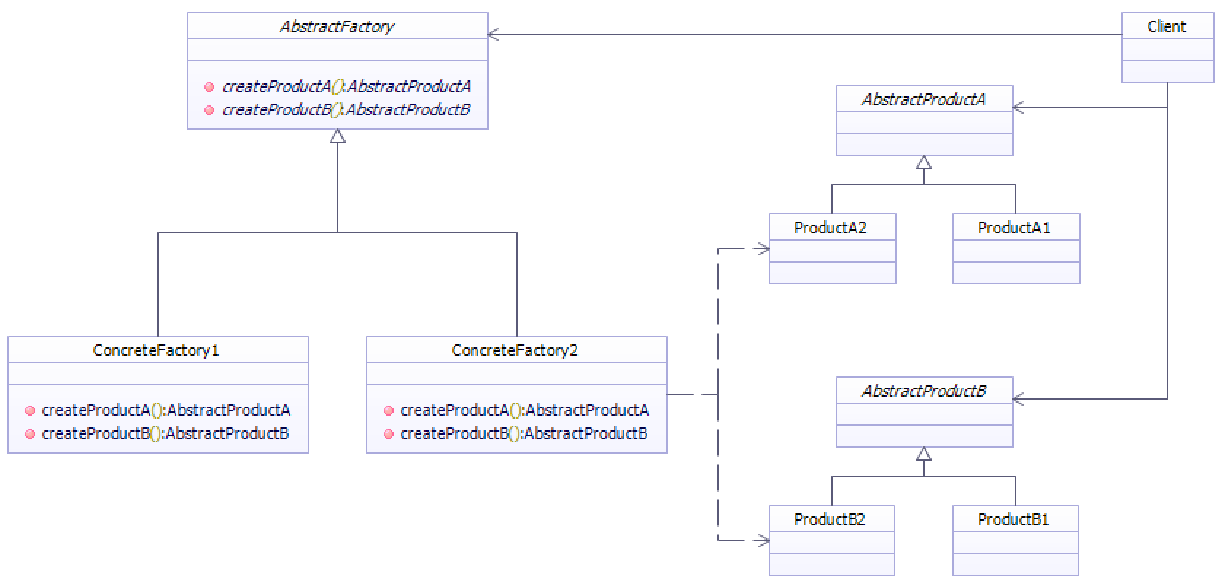
\includegraphics[width=1.0\linewidth]{arquitectura/imagenes/modeloFabAbs}
	\caption{Metamodelo Patrón Fabrica Abstracta}
	\label{fig:metamodelo fabrica abstracta}
\end{figure}

Segín esto, podemos decir que los componentes típicos del patrón Fábrica Abstracta son los siguientes:

\begin{itemize}
	\item \textbf{Cliente: }Entidad que llamará a la fábrica adecuada para crear uno de los objetos que provee dicha factoría, es decir, intentará obtener una instancia de alguno de los productos que entre en juego.
	\item \textbf{Fábrica Abstracta: }Definición de la interfaz que usarán las diferentes factorías, como mínimo, debe ofrecer un método para la obtención de cada objeto que se pueda crear
	\item \textbf{Fábricas Concretas: } Aquí se representarán las diferentes familias de los productos. Provee la instancia concreta del objeto que se encarga de crear.
	\item \textbf{Producto Abstracto: }Definirá las interfaces para la familia de productos genéricos. El cliente trabajará directamenre sobre esta interfaz, que será implementada por los diferentes productos concretos.
	\item \textbf{Producto Concreto: } Se encargará de la implementación específica de los diferentes productos.
\end{itemize}



\subsubsection{Caso de estudio}

	\begin{figure}[th!]
		\centering
		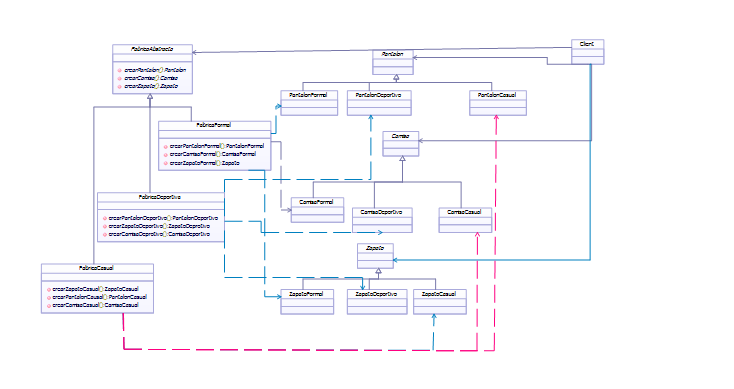
\includegraphics[width=1\linewidth]{arquitectura/imagenes/DiagramaFabricaAbstracta}
		\caption{Diagrama de clases Fabrica Abstracta}
	\end{figure}
	
	
	
	En el diagrama podemos ver que, para nuestro caso tendremos diferentes líneas de productos que podrán ser registrados en la base de datos. Para esto usamos el patrón fabrica abstracta que nos permite crear familias de productos de acuerdo a la línea establecida, además este patrón permite el escalamiento del aplicativo en forma horizontal, con lo cual, podremos a futuro adicionar otras nuevas líneas o colecciones de productos, sin necesidad de modificar las líneas ya creadas.
	
	
%%\newpage


\subsection{Método Fábrica}
\subsubsection{Modelo}
El patrón \textbf{Método Fábrica} libera al desarrollador sobre la forma correcta de crear objetos. Define la interfaz de creación de un cierto tipo de objeto, permitiendo que las subclases decidan que clase concreta necesitan instancias. Muchas veces ocurre que una clase no puede anticipar el tipo de objetos que debe crear, ya que la jerarquía de clases que tiene requiere que deba delegar la responsabilidad a una subclase. 

\begin{figure}[th!]
	\centering
	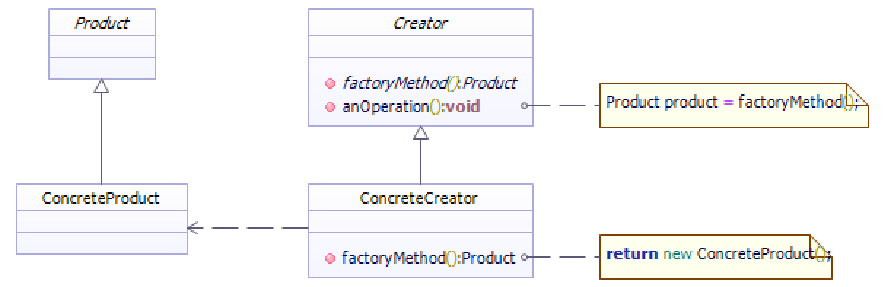
\includegraphics[width=1.0\linewidth]{arquitectura/imagenes/modeloMetFab}
	\caption{Metamodelo Patrón Método Fabrica}
	\label{fig:metamodelo metodo fabrica}
\end{figure}


Los elementos de este patrón son:
\begin{itemize}
	\item \textbf{Creador: }Declara el método de fabricación (creación), que devuelve un objeto de tipo Producto.
	\item \textbf{Creador Concreto: }Redefine el método de fabricación para devolver un producto.
	\item \textbf{Producto Concreto: }Es el resultado final. El creador se apoya en sus subclases para definir el método de fabricación que devuelve el objeto apropiado.
\end{itemize}


\subsubsection{Caso de estudio}
\begin{figure}[h!]
	\centering
	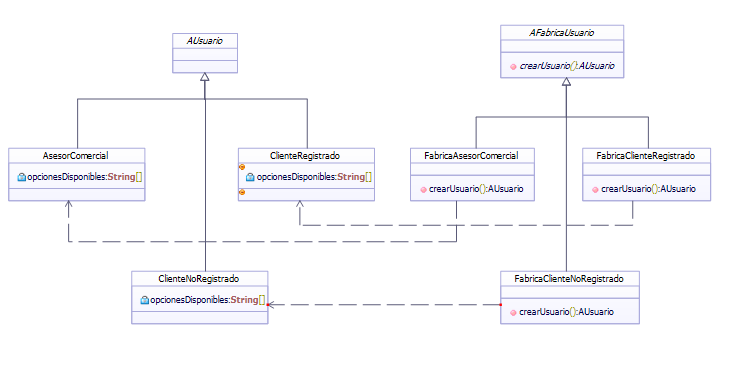
\includegraphics[width=0.7\linewidth]{arquitectura/imagenes/DiagramaMetodoFabrica}
	\caption{Modelo Patrón Método Fábrica}
\end{figure}

Para el caso de estudio se puede observar que se implemento el método fabrica para facilitar la creación del tipo de usuarios que maneja el sistema, en este caso cada usuario tiene asociados unas opciones, por ejemplo el usuario no registrado no puede realizar una compra, el usuario registrado si, entre otros, para crear un usuario para cada caso cuando se necesite y saber las opciones que este tiene asociadas se implemento este patrón.
%%\newpage

\subsection{Singleton}
\subsubsection{Modelo}
\begin{figure}[th!]
	\centering
	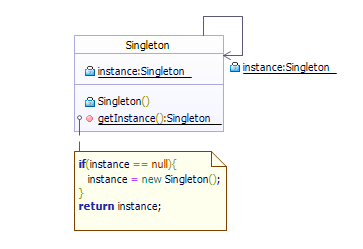
\includegraphics[width=0.7\linewidth]{arquitectura/imagenes/PatronSingelton}
	\caption{Metamodelo patron Singleton}
\end{figure}

La idea del patrón Singleton es proveer un mecanismo para limitar el número de instancias de una clase. Por lo tanto el mismo objeto es siempre compartido por distintas partes del código. Puede ser visto como una solución más elegante para una variable global porque los datos son abstraídos por detrás de la interfaz que publica la clase singleton.
Dicho de otra manera, esta patrón busca garantizar que una clase sólo tenga una instancia y proporcionar un punto de acceso global a ella.

Debe usarse cuando:
\begin{enumerate}
	\item Debe haber exactamente una instancia de una clase y deba ser accesible a los clientes desde un punto de acceso conocido.
	\item Se requiere de un acceso estandarizado y conocido públicamente.
\end{enumerate}
  

Sus usos más comunes son clases que representan objetos unívocos. Por ejemplo, si hay un servidor que necesita ser representado mediante un objeto, este debería ser único, es decir, debería existir una sola instancia y el resto de las clases deberían de comunicarse con el mismo servidor. Un Calendario, por ejemplo, también es único para todos.
\newline

Este patrón tiene una clase Singleton que define una instancia para los clientes que la acceden. Esta instancia es accedida desde un método llamado getInstancia que devuelve la instancia actual de la clase o crea una nueva en el caso de ser nula.

\subsubsection{Caso de estudio}
\begin{figure}[h!]
	\centering
	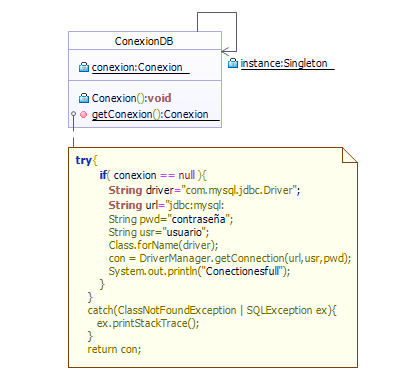
\includegraphics[width=0.7\linewidth]{arquitectura/imagenes/PatronSingeltonCasoEstudio}
	\caption{Caso de estudio patron Singleton}
\end{figure}

Para nuestro caso de estudio tenemos una clase ConexionDB que es analoga a la clase singleton, esta tiene un metodo llamado getConexion que se encarga de retornar la instancia ya creada de la clase o en el caso de que aun no exista ninguna instancia crear una nueva.\newline
La idea de  aplicar este patrón en la conexión, es para que una vez se haya establecido una conexión a la base de datos, se trabaje sobre la misma sesión y no se creen muchas conexiones dependiendo de lo que se vaya a realizar  

\newpage

\section{Patrones Estructurales}
\paragraph{Definición}
Los patrones estructurales se enfocan en como las clases y objetos se componen para formar estructuras mayores, ademas describen como las estructuras compuestas por clases crecen para crear nuevas funcionalidades de manera que se puede agregar a la estructura flexibilidad y que la misma pueda cambiar en tiempo de ejecución lo cual es imposible con una composición de clases estáticas.
\paragraph{Tipos de Patrones}
Los patrones que se encuentran en la lista de Patrones Estructurales en el enfoque GOF son:
\begin{enumerate}
	\item Bridge (Puente)
	\item Adapter (Adaptador)
	\item Composite (Componente)
	\item Decorator (Decorador)
	\item Facade (Fachada)
	\item Flyweight (Peso Ligero) 
	\item Proxy (Proxy)
\end{enumerate}

\subsection{Puente}
	
\subsubsection{Modelo}

El patrón \textbf{Bridge o Puente} desacopla una abstracción de su implementación, de manera que ambas puedan variar de forma independiente. ¿Que quiere decir exactamente esto? Una abstracción se refiere a un comportamiento que una clase debería implementar, ya sea porque esta obligada por una interface o una clase abstracta. Por otro lado, con implementación se refiere a colocarle lógica a dicha obligación. Cuando un objeto tiene unas implementaciones posibles, la manera habitual de implementación es el uso de herencias. Muchas veces la herencia se puede tornar inmanejable y, por otro lado, acopla el código cliente con una implementación concreta. 

\begin{figure}[th!]
	\centering
	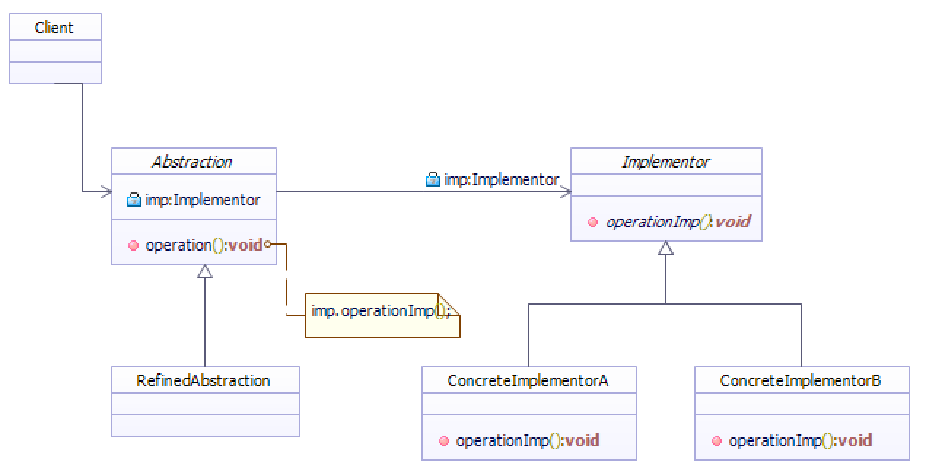
\includegraphics[width=1\linewidth]{arquitectura/imagenes/modeloPuente}
	\caption{Metamodelo Patrón Puente}
	\label{fig:puente}
\end{figure}

Este patrón busca eliminar la inconveniencia de esta solución. Las clases manejadas por este patrón son:
\begin{itemize}
	\item \textbf{Abstracción: }Define una interface abstracta. Mantiene una referencia a un objeto de tipo Implementor.
	\item \textbf{Abstracción Refinada: }Extiende la interface definida por Abstracción 
	\item \textbf{Implementador: }Define la interface para la implementación de clases. Esta interface no se tiene que corresponder exactamente con la interface de Abstraccion; de hecho, las dos interfaces pueden ser bastante diferentes entre sí. Típicamente la interface Implementador provee sólo operaciones primitivas, y Abstraccion define operaciones de alto nivel basadas en estas primitivas.
	\item \textbf{Implementador Concreto: }Implementa la interface de Implementador y define su implementación concreta.
\end{itemize}

\subsubsection{Caso de estudio}

\begin{figure}[th!]
\centering
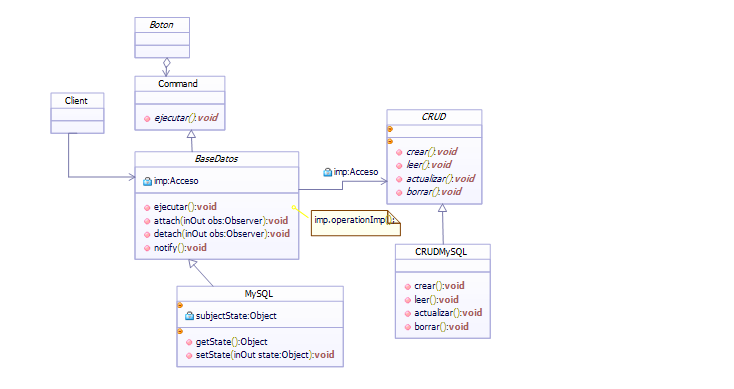
\includegraphics[width=1.0\linewidth]{arquitectura/imagenes/DiagramaComandoYPuente}
\caption{Diagrama de clases  Comando y Puente}
\end{figure}



El patrón comando utilizado en este caso permite separar y simplificar el uso de los botones y la función de cada uno en distintas opciones presentadas al usuario, para este caso particular están definidos los casos en los que el Admin crea, modifica, elimina o agrega un nuevo producto a la base de datos.
El patrón bridge, es un puente entre la abstracción de una base de datos y sus funciones con la lógica de estas funciones de acuerdo con el tipo de base de datos, puesto que la manera en que se borra, crea, agrega o modifica es diferente en cada base de datos (MySQL, Postgres, etc), de manera que en la base concreta se define el método en que cada función de la abstracción, realiza su operación. Esto permite que más adelante podamos agregar otras bases de datos a nuestro aplicativo sin la necesidad de modificar el código ya creado, y haciendo escalamiento de nuestro programa de manera horizontal.

\subsection{Fachada}
\subsubsection{Modelo}

El patrón \textbf{Facade o Fachada} busca simplificar el sistema, desde el punto de vista del cliente, proporcionando una interfaz unificada para un conjunto de subsistemas, definiendo una interfaz de nivel más alto. Esto hace que el sistema sea más fácil de usar.

\begin{figure}[th!]
	\centering
	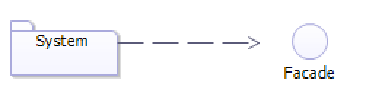
\includegraphics[width=0.6\linewidth]{arquitectura/imagenes/modeloFachada}
	\caption{Metamodelo Patrón Fachada}
	\label{fig:metamodelo patron fachada}
\end{figure}


Las clases utilizadas por este patrón son:
\begin{itemize}
	\item \textbf{Fachada: }Conoce cuales clases del subsistema son responsables de una petición. Delega las peticiones de los clientes en los objetos del subsistema.
	\item \textbf{Subsistema: }Manejar el trabajo asignado por el objeto Facade. No tienen ningún conocimiento de la Fachada (no guardan referencia de éste).
\end{itemize}


\subsubsection{Caso de estudio}
\begin{figure}[h!]
	\centering
	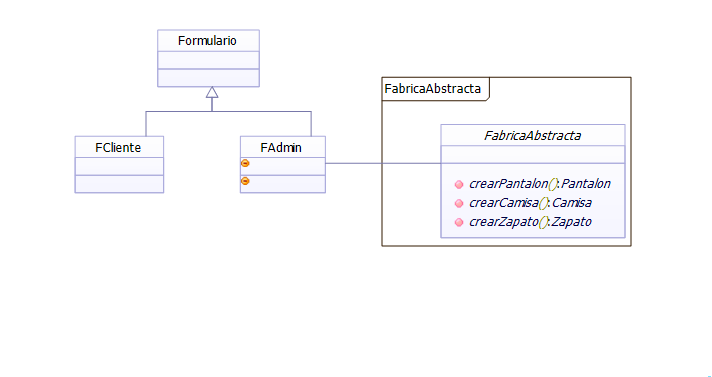
\includegraphics[width=0.8\linewidth]{arquitectura/imagenes/DiagramaFachada}
	\caption{Diagrama de clases patrón Fachada}
\end{figure}

Este patrón nos permite ocultar al cliente y al admin lo que sucede detrás del formulario que utilizan, es decir oculta la lógica del programa, la cual no es interesante para ellos, podemos incluir varios subsistemas con este patrón y dejarlos solo visibles para los que esten realmente interesados en cada uno. 
\newpage

\section{Patrones de Comportamiento}
\paragraph{Definición}
Los patrones de Comportamiento son los patrones ofrecen soluciones con respecto a la interacción y responsabilidades que hay entre objetos y clases, y las interacciones que hay entre estos ademas de los algoritmos que estos contiene.
\paragraph{Tipos de Patrones}
Los patrones que se encuentran en la lista de Patrones de Comportamiento en el enfoque GOF son:
\begin{enumerate}
	\item Command (Comando)
	\item Chain of Responsability (Cadena de responsabilidades)
	\item Iterator (Iterador)
	\item Interpreter (Interprete)
	\item Mediator (Mediador)
	\item Observer (Observador)
	\item State (Estado)
	\item Strategy (Estrategia)
	\item Template Method (Método Plantilla)
	\item Visitor (Visitante)
\end{enumerate}

\subsection{Comando}
\subsubsection{Modelo}
El patrón \textbf{Bridge o Puente} desacopla una abstracción de su implementación, de manera que ambas puedan variar de forma independiente. ¿Que quiere decir exactamente esto? Una abstracción se refiere a un comportamiento que una clase debería implementar, ya sea porque esta obligada por una interface o una clase abstracta. Por otro lado, con implementación se refiere a colocarle lógica a dicha obligación. Cuando un objeto tiene unas implementaciones posibles, la manera habitual de implementación es el uso de herencias. Muchas veces la herencia se puede tornar inmanejable y, por otro lado, acopla el código cliente con una implementación concreta. Este patrón busca eliminar la inconveniencia de esta solución.

\begin{figure}[th!]
	\centering
	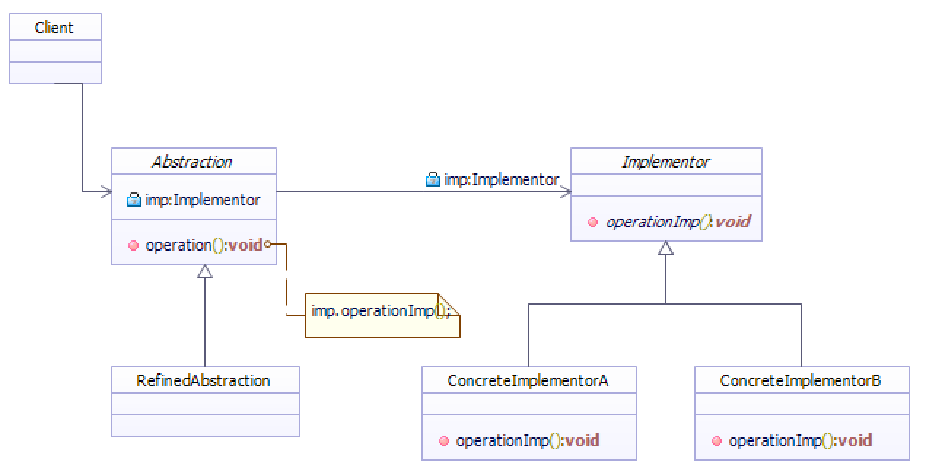
\includegraphics[width=1.0\linewidth]{arquitectura/imagenes/modeloPuente}
	\caption{Metamodelo Patrón Puente}
	\label{fig:metamodelo puente}
\end{figure}

Las clases manejadas por este patrón son:
\begin{itemize}
	\item \textbf{Abstracción: }Define una interface abstracta. Mantiene una referencia a un objeto de tipo Implementor.
	\item \textbf{Abstracción Refinada: }Extiende la interface definida por Abstracción 
	\item \textbf{Implementador: }Define la interface para la implementación de clases. Esta interface no se tiene que corresponder exactamente con la interface de Abstraccion; de hecho, las dos interfaces pueden ser bastante diferentes entre sí. Típicamente la interface Implementador provee sólo operaciones primitivas, y Abstraccion define operaciones de alto nivel basadas en estas primitivas.
	\item \textbf{Implementador Concreto: }Implementa la interface de Implementador y define su implementación concreta.
\end{itemize}



\subsubsection{Caso de estudio}


\begin{figure}[th!]
	\centering
	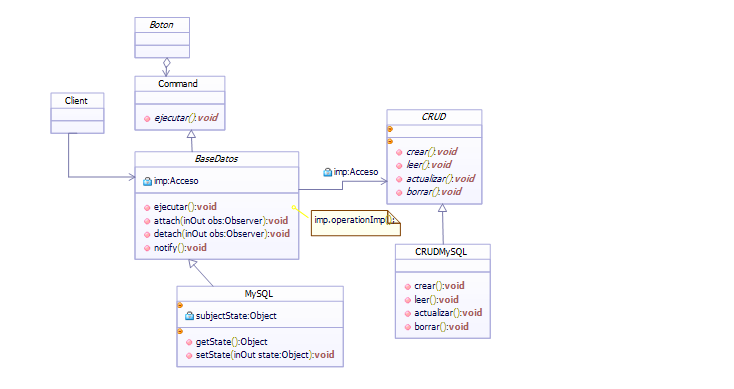
\includegraphics[width=1.0\linewidth]{arquitectura/imagenes/DiagramaComandoYPuente}
	\caption{Diagrama de clases  Comando y Puente}
\end{figure}



El patrón comando utilizado en este caso permite separar y simplificar el uso de los botones y la función de cada uno en distintas opciones presentadas al usuario, para este caso particular están definidos los casos en los que el Admin crea, modifica, elimina o agrega un nuevo producto a la base de datos.
El patrón bridge, es un puente entre la abstracción de una base de datos y sus funciones con la lógica de estas funciones de acuerdo con el tipo de base de datos, puesto que la manera en que se borra, crea, agrega o modifica es diferente en cada base de datos (MySQL, Postgres, etc), de manera que en la base concreta se define el método en que cada función de la abstracción, realiza su operación. Esto permite que más adelante podamos agregar otras bases de datos a nuestro aplicativo sin la necesidad de modificar el código ya creado, y haciendo escalamiento de nuestro programa de manera horizontal.

%%\newpage

\subsection{Iterador}
\subsubsection{Modelo}
El patrón \textbf{Iterator o Iterador} provee un mecanismo estándar para acceder secuencialmente a los elementos de una colección; define una interface que declara métodos para acceder secuencialmente a los objetos de una colección. Una clase accede a una colección a través de dicha interface.

\begin{figure}[th!]
	\centering
	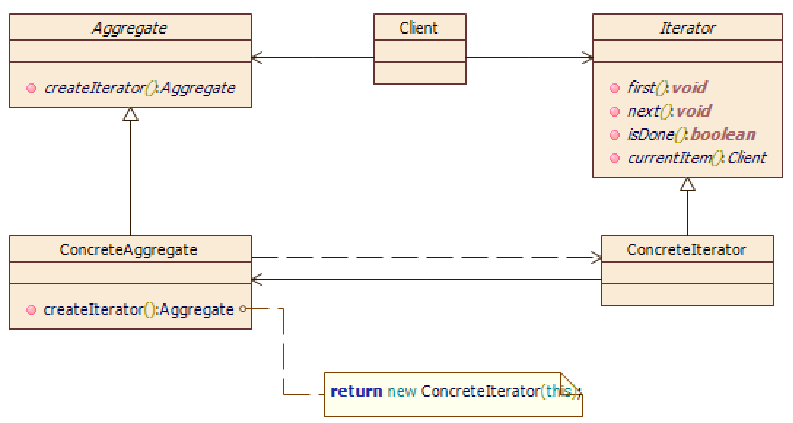
\includegraphics[width=0.8\linewidth]{arquitectura/imagenes/modeloIterador}
	\caption{Metamodelo Patrón Iterador}
	\label{fig:metamodelo patron iterador}
\end{figure}

\begin{itemize}
	\item \textbf{Agregado: }Define una interfaz para crear un objeto iterator.
	\item \textbf{Iterador: }Define la interfaz para acceder y recorrer los elementos de un agregado.
	\item \textbf{Iterador Concreto: }Implementa la interfaz del iterador y guarda la posición actual del recorrido en cada momento.
	\item \textbf{Agregado Concreto: }Implementa la interfaz de creación de iteradores devolviendo una instancia del iterador concreto apropiado.
	\item \textbf{Cliente: }Solicita recorrer una colección y lo hace siguiendo los métodos otorgados por la interfaz Iterator. 
\end{itemize}

\subsubsection{Caso de estudio}

\begin{figure}[th!]
	\centering
	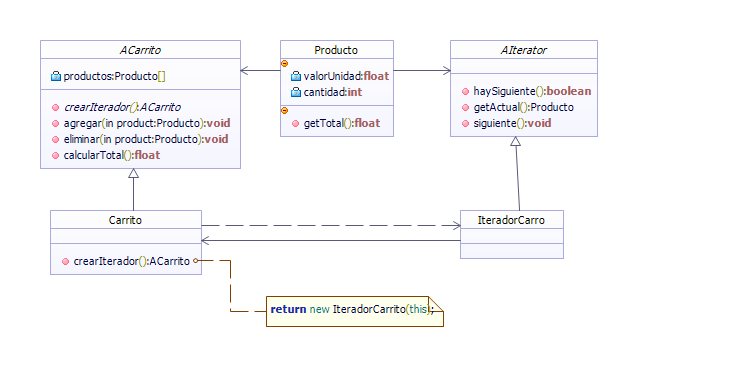
\includegraphics[width=0.9\linewidth]{arquitectura/imagenes/DiagramaIterador}
	\caption{Diagrama de clases para el patrón Iterador}
	\label{fig:patronIterador}
\end{figure}

En este caso se puede observar en la figura \ref{fig:patronIterador} que se hace uso del patrón iterador para iterar por cada uno de los elementos del carrito de compras. En este caso nuestro cliente es cada uno de los productos que pertenecen al carrito, el carrito abstracto tiene una lista de productos que son los escogidos por el cliente, cuando el cliente manipula el carrito de compras se le permite agregar o eliminar productos de este, una vez este ha decidido que desea comprar todos los elementos que tiene en el carrito es necesario para generar la factura y seguir con el proceso de pago saber el total del valor de los productos que el cliente escogió, para esto se hace uso del IteradorCarrito  el cual recorre el arreglo de productos del carrito preguntando si hay más elementos y obteniendo el valor del producto actual multiplicando el valor de la unidad por la cantidad escogida por el cliente; una vez el iterador define que no hay más elementos siguientes se puede mostrar el valor del total al cliente y continuar con el proceso de pago.



\subsection{Mediador}

\subsubsection{Modelo}
El patrón \textbf{Mediator o Mediador} define un objeto que hace de procesador central, y que se encarga coordinar las relaciones entre sus asociados o participantes. Este patrón permite la interacción de varios objetos, sin generar acoples fuertes en las relaciones. Todos los objetos se comunican con un mediador y es éste quién realiza la comunicación con el resto.

\begin{figure}[th!]
	\centering
	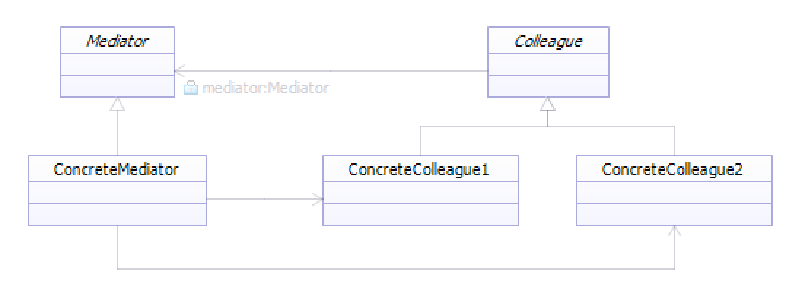
\includegraphics[width=0.8\linewidth]{arquitectura/imagenes/modeloMediador}
	\caption{Metamodelo Patrón Mediador}
	\label{fig:metamodelo patron mediador}
\end{figure}

Donde para este patrón se define que:
\begin{itemize}
	\item \textbf{Mediador: }Define una interface para comunicarse con los objetos colegas.
	\item \textbf{Mediador Concreto: }Implementa la interface y define como los colegas se comunican entre ellos.
	\item \textbf{Colega: }Define el comportamiento que debe implementar cada colega para poder comunicarse el mediador de una manera estandarizada para todos.
	\item \textbf{Colega Concreto: }Cada colega conoce su mediador, y lo usa para comunicarse con otros colegas.
\end{itemize}

%%\newpage
\subsubsection{Caso de estudio}

\begin{figure}[th!]
	\centering
	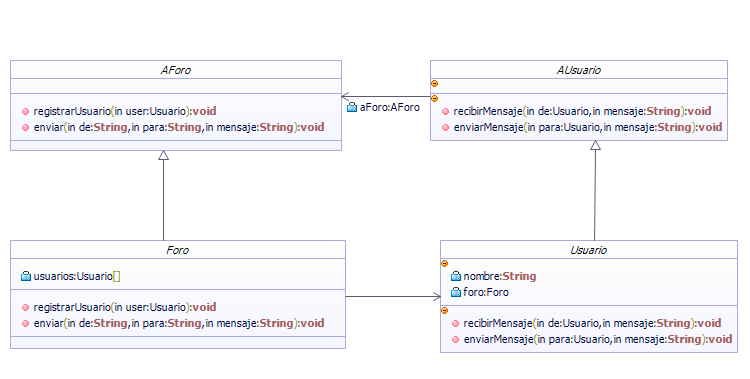
\includegraphics[width=1\linewidth]{arquitectura/imagenes/DiagramaMediator}
	\caption{Diagrama de clases Mediador}
\end{figure}

Para este caso en especifico se hace uso de patrón observador en su ejemplo más común no por simplicidad sino porque haciendo uso de este se satisface perfectamente uno de los principales requerimientos del sistema el cual es brindar un mecanismo para que a pesar de ser una tienda virtual los usuarios puedan seguir comunicandose con los asesores. \newline
En este caso se plantea una interfaz abstracta para cada usuario que tiene dos métodos, enviar y recibir mensaje, esta se implementa en cada usuario que a su vez tiene un nombre que lo identifica en el foro y le permitirá distinguirse de los demás y ademas conoce el foro. La interfaz abstracta AForo tiene dos métodos que permiten a los usuarios suscribirse al foro y el método enviar que es donde se realizara todo el proceso de registro y envio del mensaje, esta interfaz la implementa la Clase Foro que además tiene un arreglo de usuarios que son los usuarios que pertenecen al chat.



\subsection{Momento}
\subsubsection{Modelo}
\begin{figure}[th!]
	\centering
	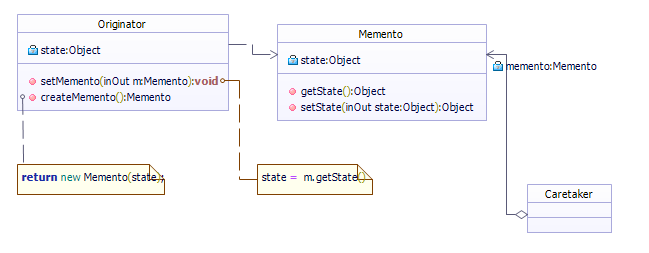
\includegraphics[width=0.9\linewidth]{arquitectura/imagenes/PatronMemento}
	\caption{Metamodelo patron memento}
	\label{fig:Metamodelo patron memento}
\end{figure}

Este patrón de diseño permite capturar y exportar el estado interno de un objeto para que luego se pueda restaurar, sin romper la encapsulación.
Su finalidad es almacenar el estado de un objeto (o del sistema completo) en un momento dado, de manera que se pueda restaurar posteriormente si fuese necesario. Para ello se mantiene almacenado el estado del objeto para un instante de tiempo en una clase independiente de aquella a la que pertenece el objeto (pero sin romper la encapsulación), de forma que ese recuerdo permita que el objeto sea modificado y pueda volver a su estado anterior.
\newline
Se usa cuando:
\begin{enumerate}
	\item Se necesite restaurar el sistema desde estados pasados.
	\item Se quiera facilitar el hacer y deshacer de determinadas operaciones, para lo que habrá que guardar los estados anteriores de los objetos sobre los que se opere (o bien recordar los cambios de forma incremental).
\end{enumerate}
Este patrón debe ser utilizado cuando se necesite salvar el estado de un objeto y tener disponible los distintos estados históricos que se necesiten.
\newline
Los componentes de este patrón son:
\begin{enumerate}
	\item Caretaker: es responsable por mantener a salvo a Memento. No opera o examina su contenido.
	\item Memento: almacena el estado interno de un objeto Originator. El Memento puede almacenar todo o parte del estado
	\item Originator: crea un objeto Memento conteniendo una fotografía de su estado interno
\end{enumerate}

\subsubsection{Caso de estudio}
\begin{figure}[h!]
	\centering
	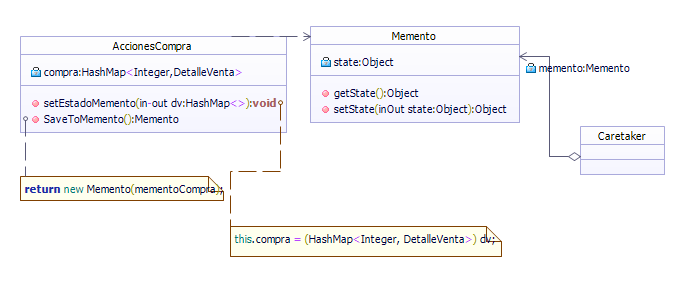
\includegraphics[width=0.7\linewidth]{arquitectura/imagenes/PatronMementoCasoEstudio}
	\caption{Caso de estudio Patrón Memento}
	\label{fig:Caso de estudio Patrón Memento}
\end{figure}

Para nuestro caso de estudio el patrón memento tiene las siguientes clases, una clase AccionesCompra, que se encarga de manejar las acciones relacionadas al carrito de compra, como agregar productos, eliminarlos, confirmar compra entre otras, cada vez que se visualizan los productos agregados al carrito, se genera un detalle de la venta, que tiene los productos y la cantidad que se va a comprar, es decir el estado del carrito, la clase memento tiene un estado que es el estado interno de la clase AccionesCompra en momento dado, y la clase CareTaker es la encarga de almacenar cada uno de los estados internos de la clase AccionesCompra y retornarlos cuando sea necesario.\newline
El objetivo del uso de este patron en estas clases, es que una vez se esten visulizando los productos agregados al carrito de compras, y se eliminen por error se pueda deshacer esta accion y retornar al estado anterior del carrito, asi mismo tambien se podra rehacer la accion devolviendo el carrito a su ultimo estado.
%%\newpage

\subsection{Observador}
\subsubsection{Modelo}

El patrón \textbf{Observer o Observador} es usado en programación para monitorear el estado de un objeto en un programa. La motivación principal de este patrón es su utilización como un sistema de detección de eventos en tiempo de ejecución.

\begin{figure}[th!]
	\centering
	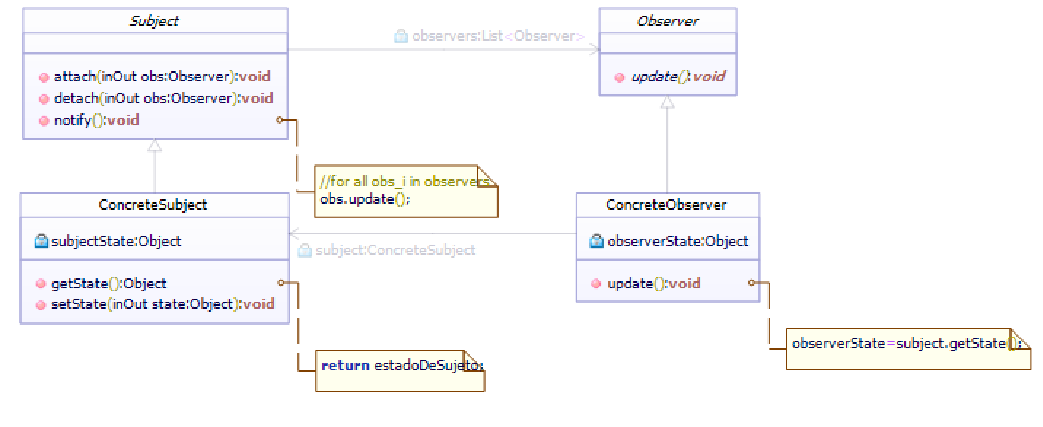
\includegraphics[width=0.8\linewidth]{arquitectura/imagenes/modeloObservador}
	\caption{Metamodelo del Patrón Observador}
	\label{fig:metamodelo patron observador}
\end{figure}

Las clases definidas para este patrón son:

\begin{itemize}
	\item \textbf{Tema: }Conoce a sus observadores y ofrece la posibilidad de añadir y eliminar observadores.
	\item \textbf{Observador: }Define la interfaz que sirve para notificar a los observadores los cambios realizados en el Tema.
	\item \textbf{Tema Concreto: }Almacena el estado que es objeto de interés de los observadores y envía un mensaje a sus observadores cuando su estado cambia.
	\item \textbf{Observador Concreto: }Mantiene una referencia a un SubjectConcreto. Almacena el estado del Tema que le resulta de interés.
\end{itemize}



\subsubsection{Caso de estudio}
	\begin{figure}[h!]
	\centering
	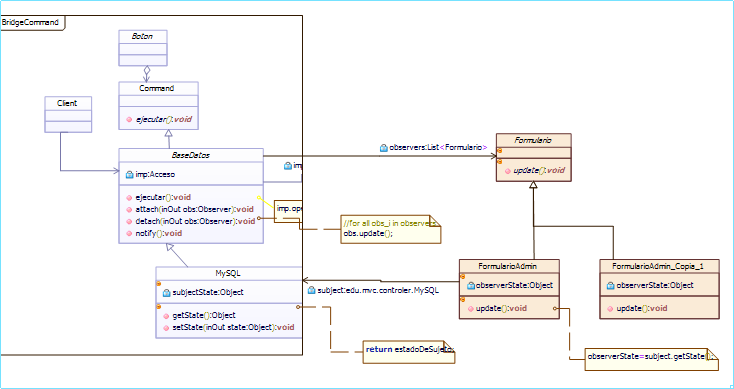
\includegraphics[width=1.0\linewidth]{arquitectura/imagenes/DiagramaObservador}
	\caption{Diagrama de clases patrón Observador}
\end{figure}



El patrón observador es utilizado en nuestro caso debido a la necesidad que tenemos de estar actualizando constantemente los datos de los productos en los formularios del Admin y el Cliente, ya sea actualizando el estado del producto en el stack, o alguna de sus características cada vez que entramos a modificarlas, este patrón nos permite facilitar esta actualización directamente en nuestra base de datos


%%\newpage

\subsection{Estado}
\subsubsection{Modelo}
\begin{figure}[th!]
	\centering
	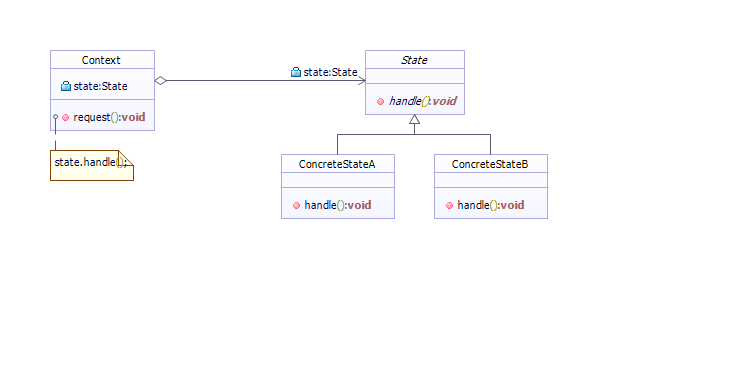
\includegraphics[width=0.7\linewidth]{arquitectura/imagenes/PatronEstado}
	\caption{metamodelo patrón estado}
	\label{fig:metamodelo patron estado}
\end{figure}
El patrón State o estado permite que un objeto modifique su comportamiento cada vez que cambie su estado interno. La intención del State es desacoplar el estado de la clase en cuestión. Las clases utilizadas son:
\begin{enumerate}
	\item Contexto:Mantiene una instancia con el estado actual Estado:Mantiene una instancia con el estado actual
	\item EstadoConcreto:Cada subclase implementa el comportamiento asociado con un estado del contexto.
\end{enumerate}  
%%\newpage

\subsubsection{Caso de estudio}
\begin{figure}[th!]
	\centering
	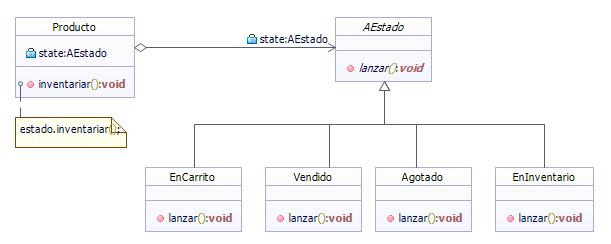
\includegraphics[width=0.7\linewidth]{arquitectura/imagenes/PatronEstadoCasoEstudio}
	\caption{}
	\label{fig:patronestadocasoestudio}
\end{figure}


En el anterior Diagrama de estados podemos ver la transición que tienen los productos desde el momento en que se cargan a la página, hasta que se realiza exitosamente una  compra, para esto nos basamos en 4 estados posibles, en inventario, en carrito, vendido, agotado, el producto empieza en un estado base de en inventario con una cantidad disponible, cuando se agrega el producto a carrito se cambia de estado a en carrito, en donde tiene dos posibles disparadores, que son desagregar de carrito y confirmar compra, si se desagrega del carrito, regresara a su estado base en inventario, si se confirma la compra cambiara de estado ha vendido, en donde se actualizara el inventario, si la cantidad comprada es igual a la disponibles en inventario, el producto quedara en un estado de agotado, si aún hay unidades disponibles volverá a un estado de inventario, a partir de ahí podemos crear una clase producto la cual podrá contener cualquiera de los 4 estados


\subsection{Estrategia}
\subsubsection{Modelo}

El patrón \textbf{Strategy o Estrategia} encapsula algoritmos en clases, permitiendo que éstos sean re-utilizados e intercambiables. En base a un parámetro, que puede ser cualquier objeto, permite a una aplicación decidir en tiempo de ejecución el algoritmo que debe ejecutar.

\begin{figure}[th!]
	\centering
	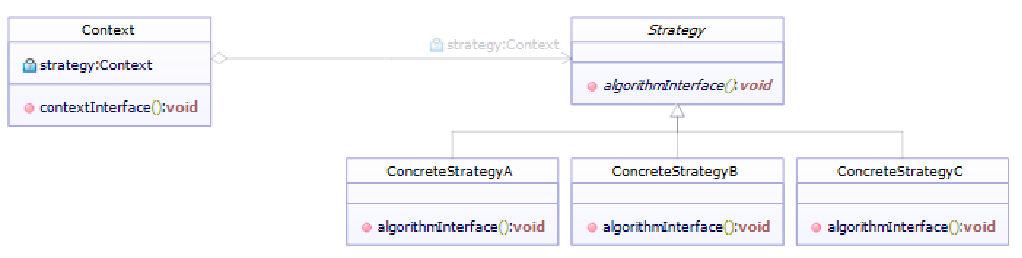
\includegraphics[width=1\linewidth]{arquitectura/imagenes/modeloEstrategia}
	\caption{Metamodelo del Patrón Estrategia}
	\label{fig:metamodelo patron estrategia}
\end{figure}

Las clases que usa este patrón son:
\begin{itemize}
	\item \textbf{Estrategia: }Declara una interfaz común a todos los algoritmos soportados.
	\item \textbf{Estrategia Concreta: }Implementa un algoritmo utilizando la interfaz Estrategia. Es la representación de un algoritmo.
	\item \textbf{Contexto: }Mantiene una referencia a Estrategia y según las características del contexto, optará por una estrategia determinada.
	\item \textbf{Cliente: }Solicita un servicio a Estrategia y este debe devolver el resultado de la Estrategia Concreta.
\end{itemize}

\subsubsection{Caso de estudio}

\begin{figure}[th!]
	\centering
	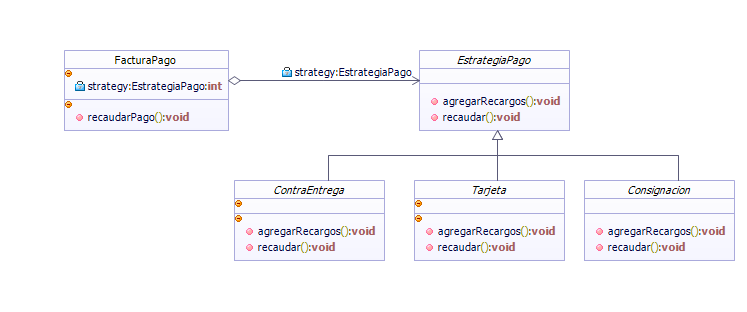
\includegraphics[width=1.0\linewidth]{arquitectura/imagenes/DiagramaEstrategia}
	\caption{Diagrama de clases patrón Estrategia}
	\label{fig:patronEstrategia}
\end{figure}


Como se puede observar en la figura \ref{fig:patronEstrategia} en este caso se aplica la estrategia para solicitar al cliente el recaudo del pago, debido a que se tienen diferentes de formas o posibilidades de pago y cada pago se hace de forma diferente, en este caso la factura solicita recaudar el  pago y conforme al método escogido por el cliente se ejecutará la estrategia correspondiente.\newline
Debido a que cada medio de pago requiere agregar recargos diferentes, como es el caso de la forma de pago de consignación y de tarjeta que requieren agregar los impuestos correspondientes, o el caso del pago a contra entrega en donde es necesario agregar el recargo del mensajero que se encargará de entregar el producto al cliente y cobrar el valor correspondiente al total.\newline
Al igual que los recargos que se agregan son diferentes, también son diferentes las formas de recaudar el pago para cada modalidad, en el caso de la contra entrega el usuario es redirigido a confirmar los datos de envió, el método de pago con tarjeta requiere comunicarse con la plataforma de pagos y la consignación redirigir al banco correspondiente.\newline
El uso de este patrón nos permite que a futuro sea posible agregar nuevas formas de pago sin tener que modificar el código y la implementación ya existente.





